\documentclass[12pt]{article}
\usepackage[russian]{babel}
\usepackage{amsmath}
\usepackage{amsfonts}
\usepackage{graphicx}
\usepackage{bm}
\newcommand{\betah}{\hat{\bm \beta}}
\newcommand{\betaa}{\bm{\beta}}
\newcommand{\epss}{\bm{\varepsilon}}
%\newcommand{\E}{\mathrm{E}}
%\newcommand{\D}{\mathrm{D}}
\newcommand{\XT}{{\bm{X}}^{\mathrm{T}}}
\newcommand{\X}{\bm{X}}
\newcommand{\y}{\bm{y}}


\begin{document}
	\title{Обучение с учителем. Регрессия. Регуляризация в регрессии. Разные подходы. Feature extraction and Feature selection}
	\author{Михайлов Дмитрий и Смирнов Иван}
	\maketitle
	
	\newpage
	\tableofcontents
	\newpage
	
	\section{Про обучение с учителем}
	
	Линейную регрессию мы уже использовали ранее. При вызове функции мы передавали модель и обучающий датасет, для каждого индивида которого уже было определено значение, которое мы хотим предсказать.
	Такой вид обучения модели называется "обучение с учителем". По сути таковым является любой алгоритм машинного обучения, где мы выдаем алгоритму как ему нужно с нашей точки зрения правильно поступить.
	
	\section{Регрессия}
	
	Пусть имеем матрицу $\mathbf{X}$ состоящую из $n$ индивидов $\mathbf{x}_i \in \mathbb{R}^p$. Предполагаем, что имеем функциональную завимость между  $\mathbf{X}$ и вектором ответов $\mathbf{y}$, состоящего из $y_i$:
	
	\begin{eqnarray}\label{regBase}  
		y_i = f(\mathbf{x}_i) + \varepsilon_i,
		\qquad 
		i=1,\ldots,n.
	\end{eqnarray}


	Где $\epsilon_i$ --- ошибка обучения или остаток. Предполагаем что они независимые, что $\mathbb{E} \varepsilon = 0$, и $\mathbb{D} \varepsilon = \sigma^2$.
	
	Задача: найти $\hat{f}$ (оценку функции регрессии $f$), чтобы для каждого индивида 	$y_i \approx \hat{f}(\mathbf{x}_i)$.
	
	\subsection{Задача оптимизации}
	
	Пусть задана модель регрессии --- параметрическое семейство функций $f(\mathbf x, \betaa)$, где $\betaa \in \mathbb{R}^p$ --- вектор параметров модели.
	
	Один из способов вычислить значения параметров модели является метод наименьших квадратов (МНК / OLS), который минимизирует среднеквадратичную ошибку между реальным значением зависимой переменной и прогнозом, выданным моделью.
	
	\begin{eqnarray}\label{ols}  
		\betah_{OLS} = \arg \min _{{\betaa}}MSE(\betaa)
	\end{eqnarray}
	
	$MSE$ --- mean squared error, выводится из \eqref{regBase}:
	
	\begin{eqnarray}\label{mse}  
		MSE(\betaa) = \frac{1}{n} \sum_{i = 1}^{n} \varepsilon_i^2 = \frac{1}{n} \sum_{i = 1}^{n}(y_i - f(\mathbf x_i, \betaa))^2
	\end{eqnarray}
	
	\subsection{Случай линейной регрессии}
	
	В модели линейной регрессии $f$ представляет собой линейную функцию, в матричном виде это:
	
	\begin{equation}\label{linRegMat}  
		\bm y = \X \betaa + \epss,
	\end{equation}
	
	Подставим (\ref{linRegMat}) в  \eqref{mse}:
	
	\begin{eqnarray}\label{linRegMSE} 
	MSE(\betaa) = \frac{1}{n} \sum_{i = 1}^{n}(y_i -\sum_{j = 1}^{p} x_{ij} \beta_j )^2 = \frac{1}{n} ||\bm y - \X \betaa||^2 = \frac{1}{n} (\bm y - \X \betaa)^T (\bm y - \X \betaa)
	\end{eqnarray}
	
	Решение при подстановке в \eqref{ols}:
	\begin{eqnarray}\label{linRegOLS}  
	\betah = (\X^T \X)^{-1} \X^{T} \bm y = \X^{-} \bm y,
	\qquad 
	\hat{\bm y} = \X \betah
	\end{eqnarray}
	
	
	Где $\X^{-}$ --- обобщённо-обратная матрица.
	
	Матрица $\X^{-}$ называется обобщённо-обратной, если:
	
	1. По аналогии с $\X^{-1}\X = \bm{I} \to \X\X^{-1}\X = \X$ и $\X^{-1}\X\X^{-1} = \X^{-1}$ выполняется $\X^{-}\X\X^{-} = \X^{-}$, $\X\X^{-}\X = \X$ 
	
	2. (Псевдообратная по Муру-Пенроузу) если по аналогии с $\X^{-1} = \X^{T}  \to (\X^{-1}\X)^T = \X^{T}(\X^{-1})^T = \X^{-1}\X$, дополнительно выполняется $\X^{-} \X = (\X^{-} \X)^T, \X \X^{-} = (\X \X^{-} )^T$	
	
	У обобщенно-обратных матриц есть следующие важные для нас свойства:
	
	1.  Если столбцы $\X$ линейно-независимы, то существует $(\X^T \X)^{-1}$ и $\X^{-} = (\X^T \X)^{-1} \X^T$
	
	2.  Пусть ищем решение $\X \betaa = \bm y$ относительно $\betaa$, если решение не единственно, то $\betaa = \X^{-} \bm y$ есть решение с минимальной нормой.
	
	
	Вычислительная проблема:  при плохой обусловленности матрицы $\X^{T} \X$ вычисление обратной к ней матрицы крайне нежелательно. Поэтому на практике лучше избегать прямого использования формул \eqref{linRegOLS}.
	
	\subsection{МНК и SVD}
	
	Пусть $\mathbf{X}=\mathbf{V}\mathbf{D}\mathbf{U^{T}}$ --- сингулярное разложение $\mathbf{X}$.
	Тогда псевдообратную к $\mathbf{X}$ матрицу легко записать в виде
	\begin{equation*}
		\mathbf{X}^{-}
		=
		\mathbf{U}\mathbf{D}^{-1}\mathbf{V}^{T}
		=
		\sum_{j=1}^{p}
		\frac{1}{\sqrt{\lambda_{j}}}
		U_{j}V_{j}^{T}.
	\end{equation*}
	Вектор МНК-решения:
	\begin{equation}\label{eq:B_SVD}
		\betah =\mathbf{X}^{-}\bm y
		=
		\sum_{j=1}^{p}
		\frac{1}{\sqrt{\lambda_{j}}}
		U_{j}(V_{j}^{\mathrm{T}} \bm y).
	\end{equation}
	Оценка $\bm y$:
	\begin{equation}\label{eq:Y_SVD}
		\hat{\bm y}
		=
		\mathbf{X}\betah
		=
		\sum_{j=1}^{p}
		V_{j}(V_{j}^{T}).
	\end{equation}
	Норма вектора коэффициентов:
	\begin{equation}\label{eq:||B||_SVD}
		||\betah||^{2}
		=
		\sum_{j=1}^{p}
		\frac{1}{\lambda_{j}}(V_{j}^{\mathrm{T}} \bm y)^{2}.
	\end{equation}
	Таким образом, имея сингулярное разложение, не приходится вычислять обратную матрицу. Эффективные численные алгоритмы, вычисляющие SVD, реализованы
	во многих стандартных математических пакетах.
	
	\section{Регуляризация}
	
	Хорошая оценка $\betah$ должна иметь низкую среднеквадратическую ошибку 
	\begin{equation*}
		\label{eq:mse}
		\mathbb{E}(\betaa - \betah)^2 = \underbrace{\mathbb D \betah}_{\text{дисперсия}} + \underbrace{(\mathbb E \betah - \betaa)^2}_{\text{смещение}}.
	\end{equation*}
	
	Несмещенная МНК-оценка не гарантирует минимизацию всей $\mathrm{MSE}$.
	Когда матрица $\bm{X}$ близка к вырожденной (это может произойти из-за наличия мультиколлинеарности или когда число предикторов $p$ почти равно числу наблюдений $n$), дисперсия $\hat{\bm \beta}$ становится большой и $\mathrm{MSE}_{\mathrm{test}}$ увеличивается.  При $p>n$ или при полностью коллинеарных признаках оценки по методу наименьших квадратов не имеют уникального решения.
	
	Введение небольшого смещения в оценке может привести к значительному уменьшению дисперсии и тем самым уменьшению $\mathrm{MSE}_{\text{test}}$.
	
	
	Регуляризация --- метод добавления некоторых дополнительных ограничений к условию с целью решить некорректно поставленную задачу или предотвратить переобучение, которое возникает, когда наша модель сильно подстраивается под данные, мы боремся с этим добавляя некоторый штраф за большие значения коэффициентов у линейной модели. Тем самым запрещаются слишком "резкие" изгибы, и предотвращается переобучение.
	
	Соответственно, необходимо добавить в целевую функцию штраф за слишком большие значения параметров. Наиболее часто используемые виды регуляризации — $L_1$ (lasso regularization или регуляризация через манхэттенское расстояние) и $L_2$ (ridge regularization или регуляризация Тихонова).
	
	\subsection{Ridge}
	Добавляем к матрице  $\X^T \X$ параметр $L_2$ регуляризации $\tau$:
	\begin{equation}\label{ridgeMatrix}
		\betah_{ridge} = (\X^T \X + \tau \bm I)^{-1} \X^T \y
	\end{equation}

	Пользуясь SVD:
	\begin{equation}\label{ridgeB}
			\betah_{ridge} =\mathbf{X}^{-}\bm y
		=
		\sum_{j=1}^{p}
		\frac{\sqrt{\lambda_{j}}}{\sqrt{\lambda_{j}}+\tau}
		U_{j}(V_{j}^{\mathrm{T}} \bm y).
	\end{equation}
	
	За счет положительного параметра $\tau > 0$ при малых $\lambda$ мы можем отделить знаменатель от нуля. Значение параметра $\tau$ выбирают на основании кросс-валидации (минимизируя ошибку на валидационной выборке).
	
	Задача в явном виде записывается как:
	\begin{equation}\label{ridgeTask1}
		\betah_{ridge} = \arg \min _{{\beta}} || \y - \X \betaa ||^2
		\qquad
		|| \betaa ||_2^2 \leq \tau
	\end{equation}

	\subsection{Lasso}
	В Lasso используется $L_1$-регуляризатор. Задача в явном виде записывается как:
	\begin{equation}\label{lassoTask1}
		\betah_{lasso} = \arg \min _{{\beta}} || \y - \X \betaa ||^2
		\qquad
		|| \betaa ||_1 \leq \tau
	\end{equation}		
	
	Lasso чаще всего обнуляет значения некоторых параметров, что в случае с линейными моделями приводит к отбору признаков.
	
	\newpage
	
	\begin{figure}[h!]
		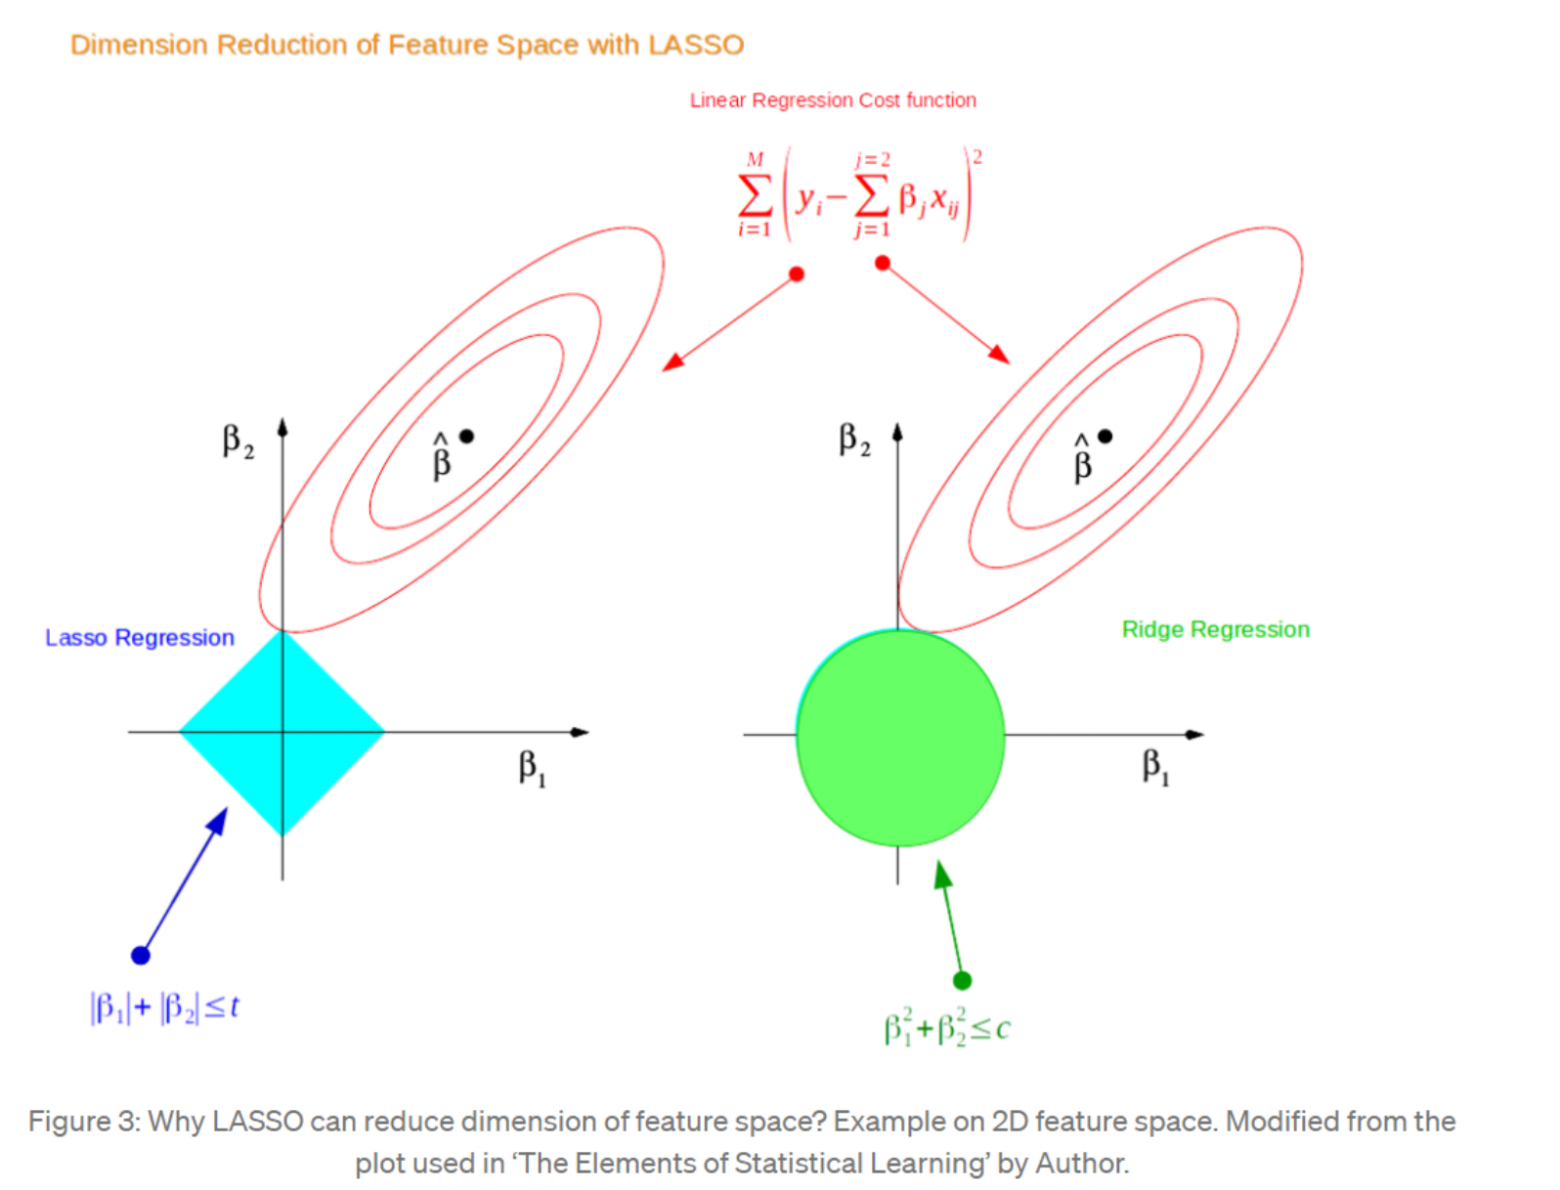
\includegraphics[width=\linewidth]{img/1}
		\caption{Сравнение lasso и ridge в случае линейной регрессии с двумя признаками}
		\label{1}
	\end{figure}
	
	В случае обычной регрессии без штрафов точка $\betah$ была бы решением задачи, но ограничение на слишком большие коэффиценты не дает нам этого сделать, вместо этого берется точка пересечения исходной модели с плоскостью ограничений. Тут мы видим, что у lasso точка пересечения $(0; \beta_{2}^{lasso})$, а у ridge  $(\beta_{1}^{ridge}; \beta_{2}^{ridge})$, соответственно lasso позволяет нам таким образом упростить модель и повысить её интерпретируемость.
	
	Однако могут быть крайние случаи в которых lasso не обнулит коэффиценты, а ridge занулит, поэтому оптимальный метод выбиается на основе кросс-валидации на конкретных данных.
	
		
	\begin{figure}[h!]
		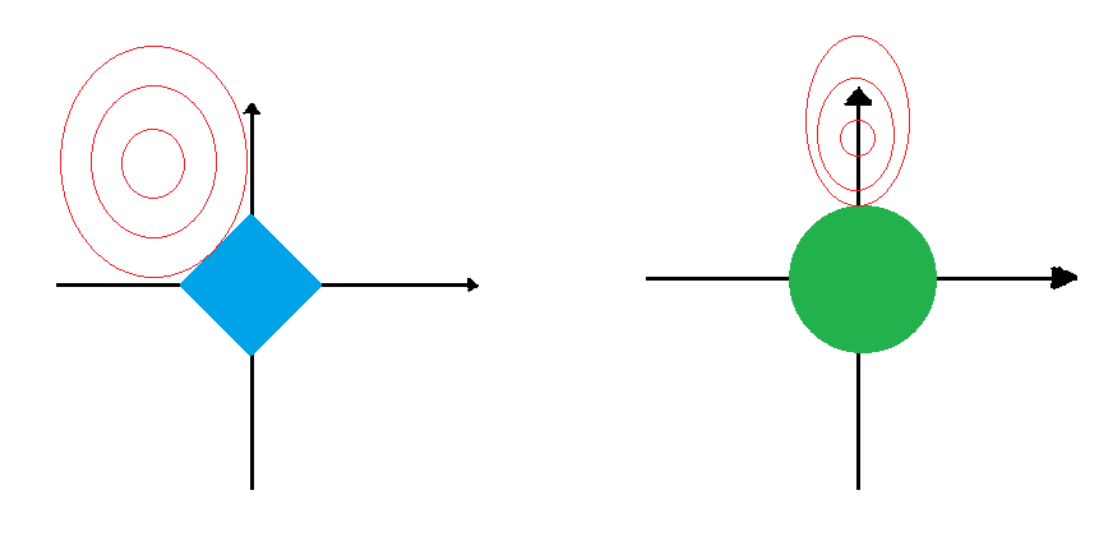
\includegraphics[width=\linewidth]{img/2}
		\caption{Случай, когда ridge лучше lasso}
		\label{2}
	\end{figure}
	
	\section{Работа с признаками}
	
	\subsection{Feature Extraction. Анализ главных компонент}
	
	Отличительной особенностью большинства наборов данных является то, что они содержат большое количество признаков, и, кроме того, эти признаки требуют много вычислительных ресурсов для их обработки. В этом случае их извлечение может быть полезно при выборе конкретных признаков, а также при объединении некоторых связанных признаков, что может уменьшить объем данных.
	
	Мы ранее уже пользовались АГК для уменьшения размерности матрицы данных, и мы также можем применить это к регрессии, чтобы улучшить модель. В методе главных компонент строится минимальное число новых признаков, по которым исходные признаки восстанавливаются линейным преобразованием с минимальными погрешностями. Этот метод также можно использовать для обнаружения аномалий и выбросов, что также улучшает качество регрессии.
	
	\subsection{Feature Selection. Информационные критерии}
	
	Как отмечалось ранее, в результате применения метода lasso получается вектор коэффициентов с большим количеством нулей, что приводит к итоговой модели с малым числом признаков. По сути, осуществляется процедура \textit{отбора признаков}.
	
			
			AIC и BIC также используются при отборе признаков. Эти критерии показывают, какая модель лучше, но не утверждают, что лучшая модель является правильной.
			
			Пусть $\mathcal L(\X; \mathcal M_i)$ --- максимум (по параметрам распределения) функции правдоподобия для модели $\mathcal M_i$, $p_i$ - число параметров в модели $i$. Тогда
			
			$$
			\mathrm{AIC}_i = 2p_i - 2\ln{\mathcal L(\X; \mathcal M_i)};
			$$
			$$
			\mathrm{BIC}_i = p_i\ln{n} - 2\ln{\mathcal L(\X; \mathcal M_i)}.
			$$
			Они представляют из себя функцию правдоподобия выборки с поправкой-штрафом, зависящей от числа параметров и размера выборки. Исходя из вида критериев, чем меньше значение, тем лучше; выбирается модель, у которой BIC или AIC наименьший.
			
	
	
		
\end{document}